\documentclass{article}
\usepackage[final]{nips_2017}
\usepackage[utf8]{inputenc} % allow utf-8 input
\usepackage[T1]{fontenc}    % use 8-bit T1 fonts
\usepackage{hyperref}       % hyperlinks
\usepackage{url}            % simple URL typesetting
\usepackage{booktabs}       % professional-quality tables
\usepackage{amsfonts}       % blackboard math symbols
\usepackage{amsmath}
\usepackage{nicefrac}       % compact symbols for 1/2, etc.
\usepackage{microtype}      % microtypography
\usepackage{graphicx}
\usepackage{subcaption}
\title{Pongfuscated: Teaching RL Pong Agents to Self-Obfuscate}

\author{
  Eli Andrew\\
  Department of Computer Science\\
  Stanford University\\
  \texttt{eyandrew@stanford.edu} \\
}

\begin{document}

\begin{center}

\includegraphics[width=3cm, height=0.7cm]{CS230}
\end{center}

\maketitle

\begin{abstract}

Deep RL methods can solve complex environments without any prior knowledge of how the environment functions. Yet, these
methods tend to need the full input data they were trained on, in order to perform well at test time. In our paper, we
attempt to modify the training of these agents, such that they focus less on certain types of input data during training,
therefore making them less susceptible to unimportant changes in those types of input data at test time. In other words, the agents learn to
self-obfuscate less informative input data during training, so that they are robust to certain obfuscations during test time. 
We trained and tested using two different model architectures, Deep-Q Learning and Policy Gradient, and obfuscated both the 
center and opponent's side of the screen. Our methods relied on using action-interest at a given input frame to weight the 
learning and action decisions for each agent for that particular input frame. We show that action-interest was effective in both the non-obfuscated 
task, and the middle of the screen obfuscation, as well as slightly effective in the opponent obfuscation task.


\end{abstract}

\section{Introduction}	
DeepMind's Atari Pong solution showed the power of RL to learn to play a game from nothing but raw pixel values. Despite the fact that no
game logic is programmed in, the agent learns how it can manipulate the environment into states with high reward. The end result is that we get an agent that understands how to interact 
and thrive in an environment, but also one that sees all input data as equal and necessary to know how to act.

In pong, this means that the agent tracks and reacts to each input frame rather than scanning for a specific type of input data and planning it's actions
accordingly. In our paper, we attempt to aide the agents in learning to self-obfuscate non-informative input data and focus more intently on
more useful input data. Using two different architectures, we introduce an action-interest mechanism that weights how the agent learns from and acts in a specific
input frame, and is intended to push the agent to learn more from, and act more in, informative frames and less from non-informative frames.

\section{Related Work}

The original work that inspired this paper was done by the DeepMind team as outlined in their famous Nature paper in 2015. This paper showed the power
of deep reinforcement learning applied to a variety of Atari pixel games, and proved that it wasn't necessary for domain knowledge to be programmed into the
agent in order for it to succeed. Furthermore, the work done by researchers at the Israel Institute of Technology and University of Cambridge on action elimination networks,
and cost-sensitive exploration inspired us to look more into ensuring that the RL-agent was taking effective actions at every state. While these papers helped to shed light
on possible ways solve our issue of learning to self-obfuscate input data, they each had a few issues that made them difficult to adopt directly. The action elimination networks
were designed to help deal with large action spaces that caused the agent to have difficulty learning what the best actions to take were. Since the action space in Pong only has three
possible actions, we decided to only use this paper as inspiration for our solution. The cost-sensitive exploration paper had great ideas about adding action costs that
inspired us to consider adding action costs to the Pong environment in order to make the agent find minimum distance paths to the ball. However, we decided to use action-interest
as a pseudo action-cost rather than adopting this paper's methods. All the related work outlined here led us to the action-interest framework we describe in this paper.

\section{Dataset and Features}
In this paper we will be focusing on using the Atari Pong OpenAI Gym environment.
The input to our algorithm will by the raw Atari frames which are $210 \times 160$
pixel images with a 128-color palette. To pre-process each frame image we will convert it into an $80 \times 80$ grey-scale
image. Finally, we will borrow an approach from the DeepMind Nature paper, where we apply our preprocessing to the last 4
frames and stack them together as input to the model.

We will then feed these input frames to a neural network that we use to parameterize Q. 
The input is an $84 \times 84 \times 4$ set of images from the last four frames of the game. The first hidden layer is a convolutional layer
with 32 filters, a kernel size of $8\times8$, a stride of 4, and a ReLU activation unit. The second hidden layer is another convolutional layer
with 64 filters, a kernel size of $4\times4$, a stride of 2, and another ReLU activation unit. A third convolutional layer is next, with 
another 64 filters, a kernel size of $3\times3$, a stride of 1, and another ReLU. Finally, we have a fully connected layer with 512 units
and and 4 output units, one for each possible action. See Fig. 1 for more a diagram of the architecture.

\begin{figure}
  \centering
  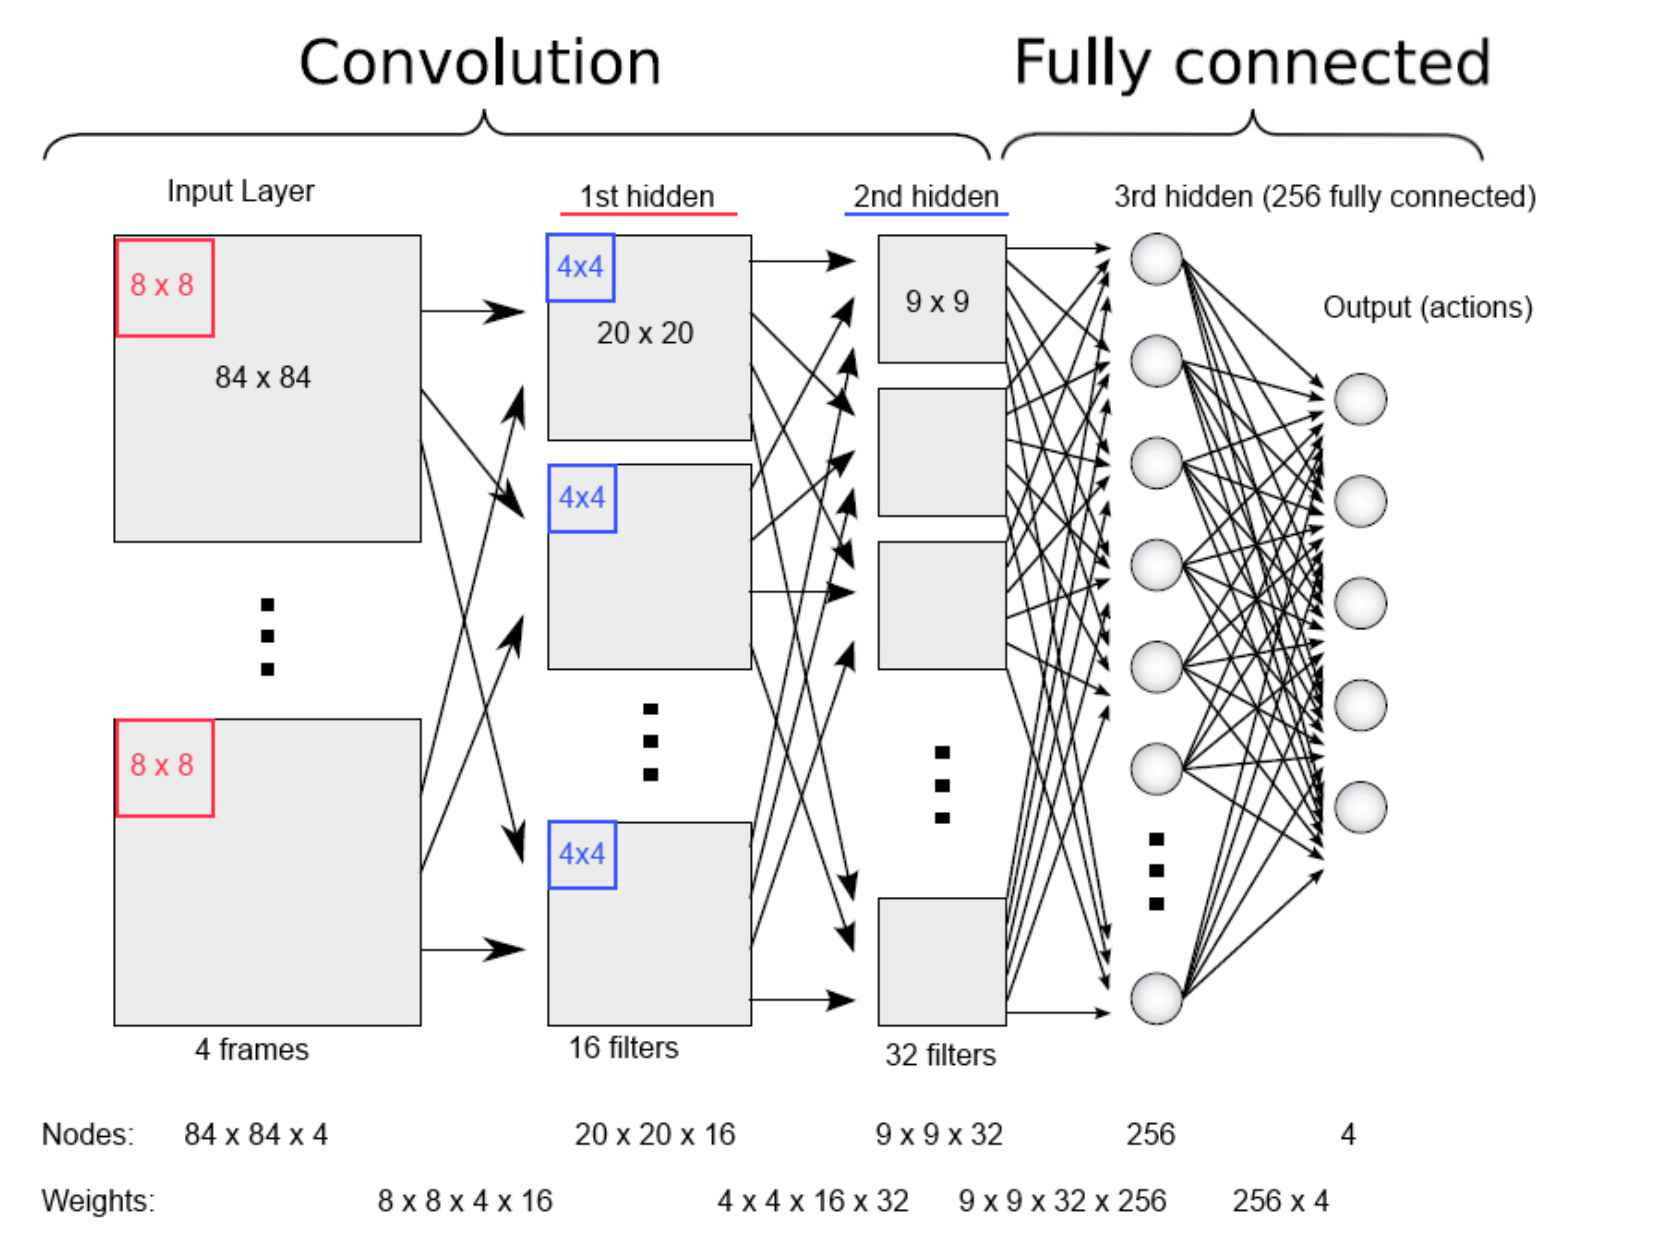
\includegraphics[width=12cm, height=10cm]{nn_diagram}
  \caption{Deep Q-Network Architecture}
  \label{fig:deepQ}
\end{figure}

We will also use a different architecture to directly learn a policy rather than to parameterize Q. This network will directly determine our policy
and will be trained using a method known as Policy Gradient. The network will be a simple two-layer network that produces one output value:
the probability of going up. This network is inspired by the article from Andrej Karpathy, and the original architecture can be
seen in Figure 2.

\begin{figure}
  \centering
  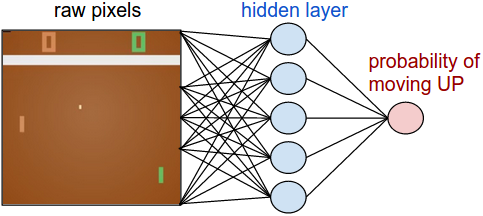
\includegraphics[width=10cm, height=5cm]{policy}
  \caption{Policy Network Architecture} 
  \label{fig:policy}
\end{figure}

While the agent trained in the DeepMind paper was seeking to maximize total reward, which meant winning as many points as possible, our
agent will be trained to not only maximize total reward, but also to understand where to focus its attention well enough to play with an obfuscated
part of the screen. The reasoning behind this modified goal is that parts of the screen in Pong contain unnecessary information
for an agent that truly understands how the game works. As long as the remaining parts of the screen contain enough information to see the velocity of the 
ball, the agent should be able to learn where the final location of the ball will be when it reaches it's side. 

\section{Methodology and Experiments}

\subsection{Action Interest Mechanism}

The main contribution of this paper is the idea of incentivizing the agent to learn from the most important parts of the input data, and
to not be overly reliant on input data that is un-necessary for the task. The question we then had to answer, was how to express a general
method for identifying areas of the input data that were more or less important for the goal of the game.

Using Pong as our environment, we can identify two potential areas of input data that are less important, and frankly not necessary for a
successful agent to consider. The first of these areas is some portion of the middle of the screen, because if the information about where the ball
will end up is encoded in the first few frames of the input after the ball leaves the opponents paddle. This type of obfuscation can be seen in Figure 3a. 
The second, maybe less obvious area, is the opponents side of the screen. Again, this is not necessary input data given that we will be able to detect 
where the ball will end up, and have enough time to move there, even without witnessing the original path of the ball. This type of obfuscation can be seen in Figure 4a.

\begin{figure}
  \centering
  \begin{subfigure}{.5\textwidth}
    \centering
    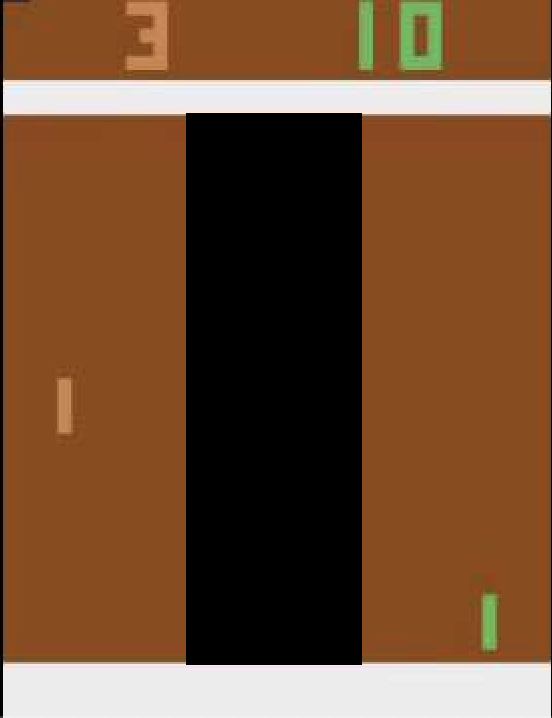
\includegraphics[width=.4\linewidth]{obfuscated_middle.png}
    \caption{Obfuscated Middle}
    \label{fig:sub1}
  \end{subfigure}%
  \begin{subfigure}{.5\textwidth}
    \centering
    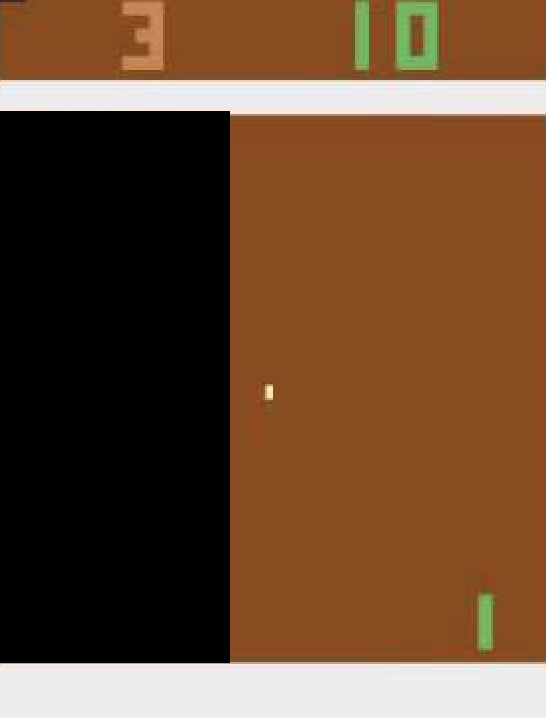
\includegraphics[width=.4\linewidth]{obfuscated_op.png}
    \caption{Obfuscated Opponent}
    \label{fig:sub2}
  \end{subfigure}
  \caption{Types of Obfuscated Input Data}
  \label{fig:obfuscated}
\end{figure}


In order to identify the regions to be self-obfuscated, we use an action-interest mechanism defined as how inclined the agent is to take one action over all
others for that particular input frame. The formula for the action-interest weight for a given input frame is:
\begin{gather*}
  A_{frame} = \frac{\max_{actions}(P_{action})}{\sum\limits_{i=0}^{n_{actions}}P_{action_i}}
\end{gather*}

This gives a weighting of how interested the agent is in a particular action versus all of the others. 

\subsection{Simple Pong Experiment}

A Simple Pong experiment was created in order to gain intuition about the problem in a much simpler environment.
In the Simple Pong experiment the game is only two pixels high and 10 pixels wide, and the paddle is only 1 pixel
by one pixel. In order to make the path of the ball as easy to learn as possible, we have the ball appear randomly in 
one of the two rows, and then continue in the same row until reaching the paddle. Once the ball reaches the paddle it is
regenerated in the same way as it started. The agent receives $+1$ for having the paddle hit the ball and $-1$ for missing the
ball.

Because this environment had a small finite number of states, we used a simple tabular Q-learning approach to solve it. The Q-values
for different states in this environment shed light on the fact that action-interest was low in different portions of the screen. 

\subsection{Baseline Experiments}
To serve as a baseline, we trained the existing DeepMind Deep-Q network on the Atari Pong OpenAI environment. This network can 
achieve great results and scores around 13-15 points on non-occluded input frames after training for 5 million steps also on non-occluded input frames.
The Policy Gradient network was trained locally and achieved an average score of around 3 points.

\subsection{Middle Obfuscation}
We then modified our code to obfuscate the input images based on a given obfuscation width. The obfuscation width is defined as how many columns of pixels
we obfuscate from the middle of the screen. For example, with an obfuscation of 2 we would be be blocking out the middle 4 columns of the screen.
For our experiments we were dealing with a screen width of 80 pixels, and we used occlusion widths of 20 and 10 pixels.

The architecture was then run through the obfuscation challenge twice: once with the original model, and once with a model
using the action-interest mechanism.

\subsection{Opponent Obfuscation}
The same obfuscation logic was used to then obfuscate the opponent's side of the screen, this time using the far left of the screen
as our reference and then blocking out the columns to the right. For example, with an obfuscation of 2 we would be blocking out the
left 4 pixel columns on the screen.

The architecture was again run through the modified obfuscation challenge twice. The same occlusion widths were used for these experiments as well.


\section{Results and Discussion}

Due to limitations in training time costs (could not afford the credits), the Deep-Q network architecture could not be trained for all the
obfuscation experiments with and without action-interest. The Policy Gradient network was, however, able to be trained and tested for all situations
and the results are summarized in Figure 4.

\begin{figure}
  \centering
  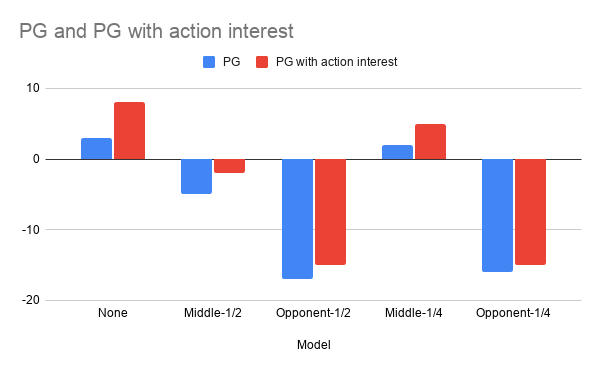
\includegraphics[width=15cm, height=10cm]{ai_plot.png}
  \caption{Obfuscation Experiments with and without Action-Interest} 
  \label{fig:actioninterest}
\end{figure}

These results show two main very interesting insights: action-interest is a somewhat effective way to mitigate the effects of
non-informative input regions marked by low interest in any particular action, and the effects of opponent obfuscation are significantly
more detrimental to performance than middle obfuscation. Furthermore, action-interest is noticeably less helpful when applied to opponent
obfuscation as compared to middle obfuscation.

This likely shows us that the agent has learned a strategy that is mainly based around initial path planning of the ball off the opponents racket.
As a result, when we obfuscate the opponent's side of the screen our agent's performance is significantly worse than when we obfuscate the middle of the
screen. In addition, since the agent utilizes the opponent's side of the screen more, the action-interest is much higher in that region than in the
middle of the screen, which makes the addition of action-interest not nearly as effective as it was for the middle of the screen obfuscation.
This also shows that the middle of the screen is an area of high action \textit{indifference} which can have it's effects mitigated by introducing
action-interest into the learning and acting algorithm. 


\section{Conclusions and Future Work}

In conclusion, our work has identified that certain regions of the input data in the Pong environment have lower utility marked by 
the agent's indifference to taking actions. We have proposed a slightly modified learning mechanism that takes into account the level of action-interest
that the agent has for that particular input frame, and shown that it improves the baseline (non-obfuscated) environment, the middle-obfuscated environment,
as well as slightly in the opponent-obfuscated environment. Our hope for future work is that we will be able to continue expanding the ability of agents to
self-obfuscate certain regions of the input data in order to make them less susceptible to non-important changes to the input data.

\section*{References}
\medskip
\small
[1] Volodymyr Mnih et al. ``Human-level control through deep reinforcement learning." In: {\it Nature}
518.7540 (2015), pp. 529-533 

[2] Volodymyr Mnih et al. ``Playing Atari With Deep Reinforcement Learning.'' In: {\it NIPS Deep Learning
Workshop.} 2013. 

[3] Karpathy, Andrej. ``Deep Reinforcement Learning: Pong from Pixels.'' {\it Andrej Karpathy Blog},
31 May 2016, {\it karpathy.github.io/2016/05/31/rl/}

[4] Korjus, Kristjan. ``Artificial Intelligence that plays Atari video games: How did DeepMind do it?'' {\it University of Tartu},
10 May 2015, {\it https://www.infoq.com/presentations/deepmind-q-network/}

[5] Hausknecht et al. ``Deep Recurrent Q-Learning for Partially Observable MDPs'' {\it University of Texas at Austin}

[6] Kim et al. ``Cost-Sensitive Exploration in Bayesian Reinforcement Learning'' {\it University of Cambridge}

[7] Zahavy et al. ``Learn What Not to Learn: Action Elimination with Deep Reinforcement Learning'' {\it Technion - Israel Institute of Technology}

\end{document}